%%%%%%%%%%%%%%%%%%%%%%%%%%%%%%%%%%%%%%%%%
% Short Sectioned Assignment LaTeX Template Version 1.0 (5/5/12)
% This template has been downloaded from: http://www.LaTeXTemplates.com
% Original author:  Frits Wenneker (http://www.howtotex.com)
% License: CC BY-NC-SA 3.0 (http://creativecommons.org/licenses/by-nc-sa/3.0/)
%%%%%%%%%%%%%%%%%%%%%%%%%%%%%%%%%%%%%%%%%

%----------------------------------------------------------------------------------------
%	PACKAGES AND OTHER DOCUMENT CONFIGURATIONS
%----------------------------------------------------------------------------------------

\documentclass[paper=a4, fontsize=11pt]{scrartcl} % A4 paper and 11pt font size

% ---- Entrada y salida de texto -----

\usepackage[T1]{fontenc} % Use 8-bit encoding that has 256 glyphs
\usepackage[utf8]{inputenc}
%\usepackage{fourier} % Use the Adobe Utopia font for the document - comment this line to return to the LaTeX default

% ---- Idioma --------

\usepackage[spanish, es-tabla]{babel} % Selecciona el español para palabras introducidas automáticamente, p.ej. "septiembre" en la fecha y especifica que se use la palabra Tabla en vez de Cuadro

% ---- Otros paquetes ----

\usepackage{url} % ,href} %para incluir URLs e hipervínculos dentro del texto (aunque hay que instalar href)
\usepackage{amsmath,amsfonts,amsthm} % Math packages
%\usepackage{graphics,graphicx, floatrow} %para incluir imágenes y notas en las imágenes
\usepackage{graphics,graphicx, float} %para incluir imágenes y colocarlas

% Para hacer tablas comlejas
%\usepackage{multirow}
%\usepackage{threeparttable}

%\usepackage{sectsty} % Allows customizing section commands
%\allsectionsfont{\centering \normalfont\scshape} % Make all sections centered, the default font and small caps

\usepackage{fancyhdr} % Custom headers and footers
\pagestyle{fancyplain} % Makes all pages in the document conform to the custom headers and footers
\fancyhead{} % No page header - if you want one, create it in the same way as the footers below
\fancyfoot[L]{} % Empty left footer
\fancyfoot[C]{} % Empty center footer
\fancyfoot[R]{\thepage} % Page numbering for right footer
\renewcommand{\headrulewidth}{0pt} % Remove header underlines
\renewcommand{\footrulewidth}{0pt} % Remove footer underlines
\setlength{\headheight}{13.6pt} % Customize the height of the header

\numberwithin{equation}{section} % Number equations within sections (i.e. 1.1, 1.2, 2.1, 2.2 instead of 1, 2, 3, 4)
\numberwithin{figure}{section} % Number figures within sections (i.e. 1.1, 1.2, 2.1, 2.2 instead of 1, 2, 3, 4)
\numberwithin{table}{section} % Number tables within sections (i.e. 1.1, 1.2, 2.1, 2.2 instead of 1, 2, 3, 4)

\setlength\parindent{0pt} % Removes all indentation from paragraphs - comment this line for an assignment with lots of text

\newcommand{\horrule}[1]{\rule{\linewidth}{#1}} % Create horizontal rule command with 1 argument of height


%----------------------------------------------------------------------------------------
%	TÍTULO Y DATOS DEL ALUMNO
%----------------------------------------------------------------------------------------

\title{	
	\normalfont \normalsize 
	\textsc{\textbf{Planificación y Gestión de Proyectos Informáticos (2018-2019)} \\ Máster Profesional de Ingeniería Informática \\ Universidad de Granada} \\ [25pt] % Your university, school and/or department name(s)
	\horrule{0.5pt} \\[0.4cm] % Thin top horizontal rule
	\huge Estimación de costes \\ % The assignment title
	\horrule{2pt} \\[0.5cm] % Thick bottom horizontal rule
}

\author{Alejandro Campoy Nieves \\ Luis Gallego Quero} % Nombre y apellidos y correo
\date{\normalsize\today} % Incluye la fecha actual
\usepackage{graphicx}
\usepackage{hyperref} % Para añadir los hiperenlaces.
\usepackage{eurosym} % Para incluir el símbolo del euro


%----------------------------------------------------------------------------------------
% DOCUMENTO
%----------------------------------------------------------------------------------------

\begin{document}
\maketitle % Muestra el Título

\newpage %inserta un salto de página

\tableofcontents % para generar el índice de contenidos

\listoffigures

\listoftables	

\newpage		
 
\section{Estimación por descomposición funcional}

\begin{table}[H]
	\begin{center}
		\begin{tabular}{|c||c|}
			\hline 
			Módulo & Esfuerzo estimado \\
			\hline \hline
			Documentación inicial & 1pm \\ \hline
			Base de datos & 2pm \\ \hline
			Deep Learning & 2pm \\ \hline
			Despliegue local & 2pm \\ \hline
			Primer refinamiento & 3pm \\ \hline
			Integración hospital & 2pm \\ \hline
			Segundo refinamiento & 3pm \\ \hline
			\textbf{Total} & \textbf{15pm} \\ \hline
		\end{tabular}
		\caption{Estimación por descomposición funcional}
		\label{tabla:funcional}
	\end{center}
\end{table}

Costes laborales: 1700 \euro/pm\\
Estimación: 1700 \euro/pm * 2p * 15pm = \textbf{51000 \euro}

\section{Estimación por descomposición de actividades}

\begin{table}[H]
	\begin{center}
		\begin{tabular}{|c|c|c|c|c|c||c|}
			\hline 
			Módulo & Plan & Análisis & Diseño & Código & Test & \textbf{Total} \\
			\hline \hline
			Documentación inicial & & 0.6 & 0.2 & 0 & 0 & \textbf{0.8}  \\ \hline
			Base de datos & & 0.5 & 0.1 & 0.1 & 0.1 & \textbf{0.8}  \\ \hline
			Deep Learning & & 1 & 0.3 & 1.2 & 0.8 & \textbf{3.3}  \\ \hline
			Despliegue local & & 0.8 & 0.2 & 0.8 & 0.5 & \textbf{2.3}  \\ \hline
			Primer refinamiento & & 0.6 & 0.3 & 1.4 & 0.5 & \textbf{2.8}  \\ \hline
			Integración hospital & & 1 & 0.2 & 0.5 & 1.5 & \textbf{3.2}  \\ \hline
			Segundo refinamiento & & 0.8 & 0.2 & 0.6 & 1.5 & \textbf{3.1}  \\ \hline
			\textbf{Total} & \textbf{0.25} & \textbf{5.3} & \textbf{1.5} & \textbf{4.6} & \textbf{4.9} & \textbf{16.3}  \\ \hline
			\textbf{    \%} & \textbf{1.53\%} & \textbf{32.51\%} & \textbf{9.2\%} & \textbf{28.22\%} & \textbf{30.06\%} & \textbf{}  \\ \hline
		\end{tabular}
		\caption{Estimación por descomposición de actividades}
		\label{tabla:actividades}
	\end{center}
\end{table}

Costes laborales: 1700 \euro/pm \\
Estimación: 1700 \euro/pm * 2 * 16.3 = \textbf{55420 \euro}

\section{Estimación del tamaño del proyecto (KLOC)}

\begin{table}[H]
	\begin{center}
		\begin{tabular}{|c||c|}
			\hline 
			Módulo & Tamaño estimado \\
			\hline \hline
			Documentación inicial & 1 KLOC \\ \hline
			Base de datos & 2 KLOC \\ \hline
			Deep Learning & 3 KLOC \\ \hline
			Despliegue local & 4 KLOC \\ \hline
			Primer refinamiento & 3 KLOC \\ \hline
			Integración hospital & 0.8 KLOC \\ \hline
			Segundo refinamiento & 3 KLOC \\ \hline
			\textbf{Total} & \textbf{16.8 KLOC} \\ \hline
		\end{tabular}
		\caption{Estimación del tamaño del proyecto (KLOC)}
		\label{tabla:tamaño}
	\end{center}
\end{table}

KLOC : Miles de líneas de código \\
Estimación : 1700 \euro/persona * 2 personas * 16.8 KLOC(1\euro/LOC) = \textbf{57120 \euro}

\section{Estimación del tamaño del proyecto (FP)}

\begin{table}[H]
	\begin{center}
		\begin{tabular}{|c||c|c|c|c|c|c|}
			\hline 
			Módulo & o & m & p & est. & peso & \textbf{fp} \\
			\hline \hline
			Documentación inicial & 5 & 10 & 15 & 10 & 3 & \textbf{30}  \\ \hline
			Base de datos & 10 & 17 & 18 & 15 & 4 & \textbf{60}  \\ \hline
			Deep Learning & 15 & 17 & 22 & 18 & 4 & \textbf{72}  \\ \hline
			Despliegue local & 14 & 16 & 18 & 16 & 2 & \textbf{32}  \\ \hline
			Primer refinamiento & 16 & 21 & 26 & 21 & 4 & \textbf{84}  \\ \hline
			Integración hospital & 12 & 14 & 16 & 14 & 2 & \textbf{28}  \\ \hline
			Segundo refinamiento & 19 & 23 & 27 & 23 & 5 & \textbf{115}  \\ \hline
			\textbf{Total} & & & & & & \textbf{421}  \\ \hline
		\end{tabular}
		\caption{Estimación del tamaño del proyecto (FP)}
		\label{tabla:FP}
	\end{center}
\end{table}


$FP_{estimado} = 1.17 * FP_{real} = 492.57$ \\
Productividad: 20 FP/pm = 40 FP/m \\
Costes laborales: 4000 \euro (\textasciitilde{}100\euro/FP) \\
Estimación: 492.57*100 = \textbf{49257 \euro} 

\section{Estimación con herramientas software: Construx Estimate}

\begin{figure}[H]
	\centering
	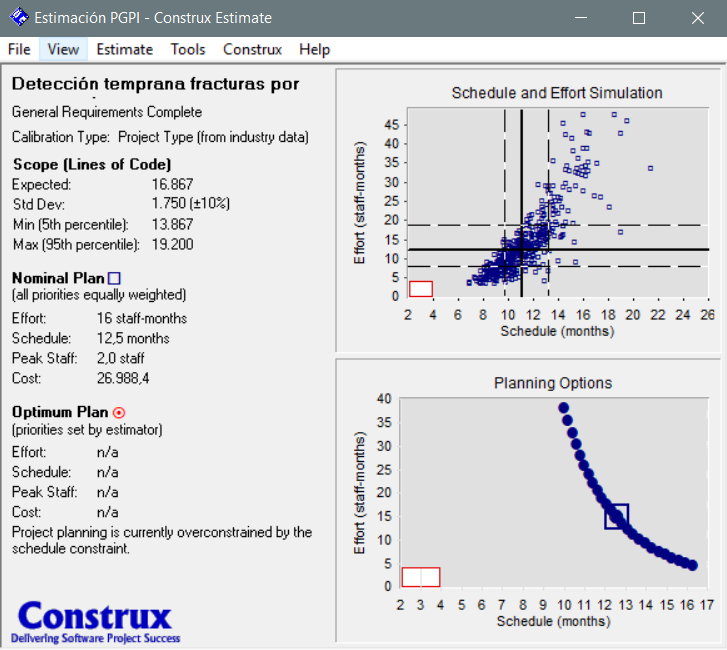
\includegraphics[scale=0.7]{figuras/estimate.png}
	\caption{Resultados obtenidos con la herramientas software Construx Estimate.} 
	\label{fig:estimate}
\end{figure}

En la estimación realizada en Construx obtenemos una estimación casi la mitad de inferior respecto a las estimaciones realizadas hasta ahora. Quizás, una de las razones principales, sea la poca parametrización que nos permite esta herramienta software y, por tanto, la poca proximidad real a la definición real de nuestro proyecto.

\section{Estimación con modelos empíricos}

\subsection{COCOMO II}

\begin{figure}[H]
	\centering
	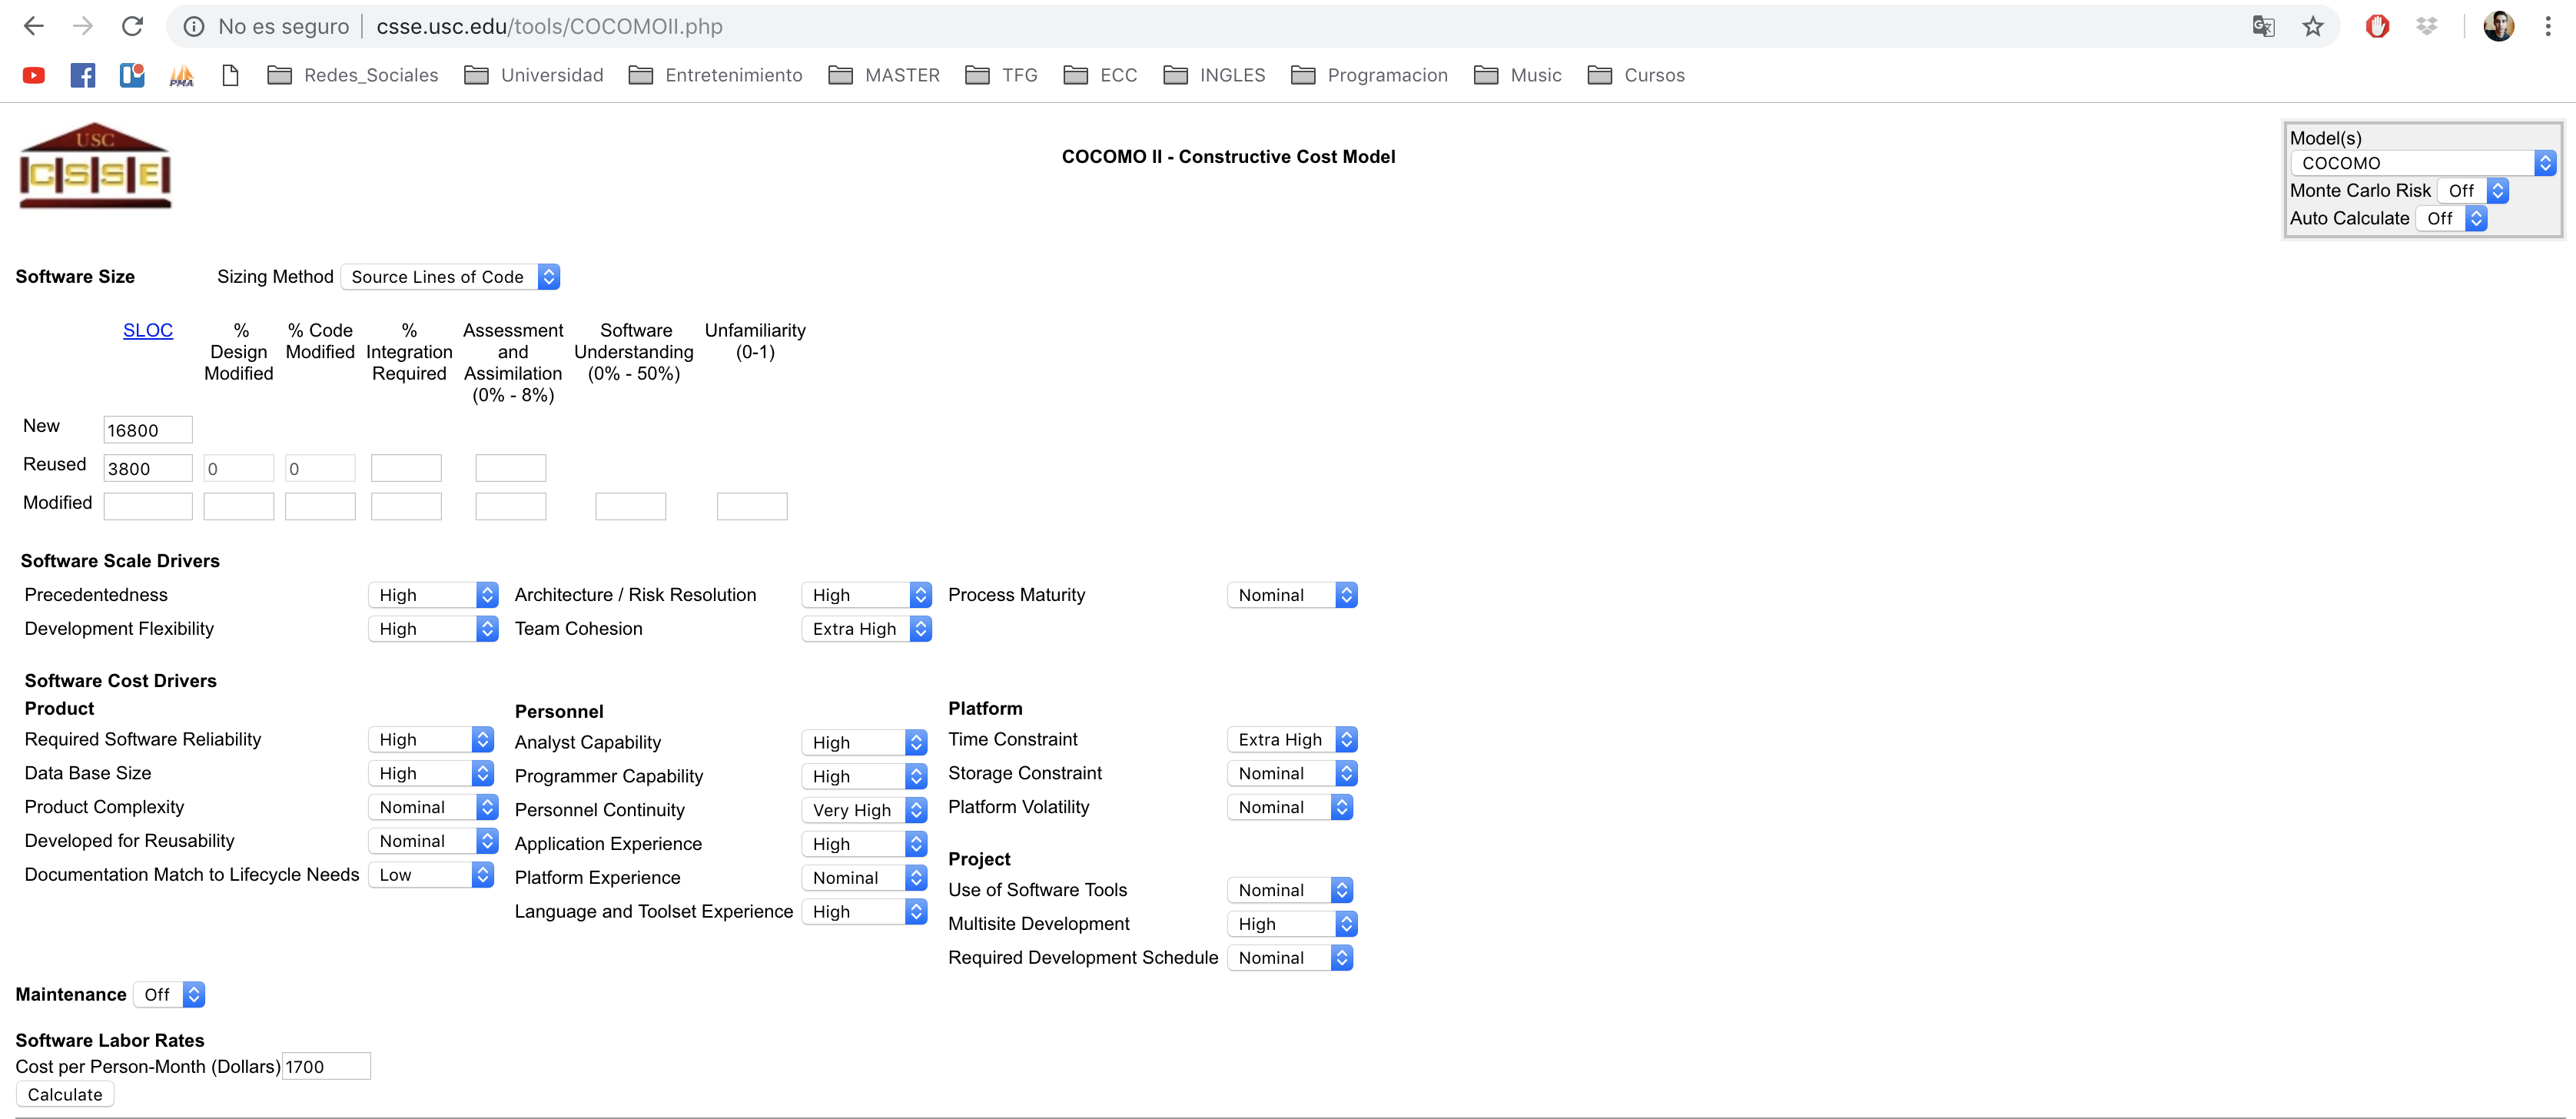
\includegraphics[scale=0.29]{figuras/cocomo1.png}
	\caption{Parámetros para COCOMO II en el proyecto.} 
	\label{fig:cocomo1}
\end{figure}

\begin{figure}[H]
	\centering
	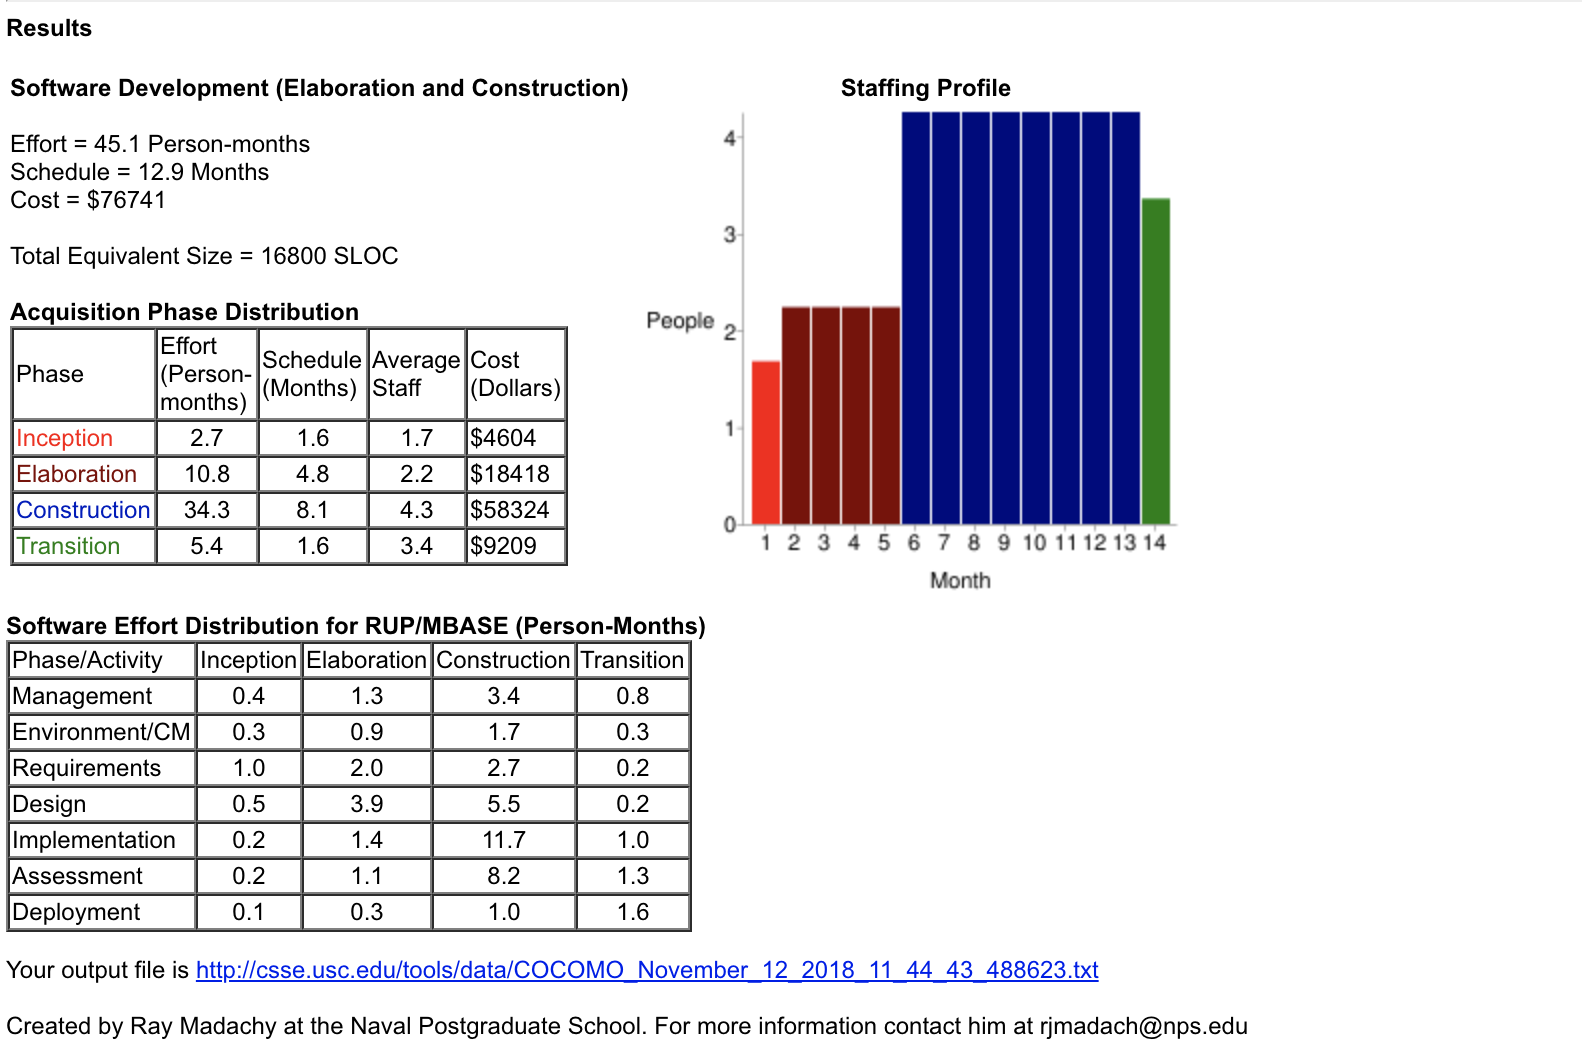
\includegraphics[scale=0.45]{figuras/cocomo2.png}
	\caption{Salidas obtenidas para COCOMO II en el proyecto.} 
	\label{fig:cocomo2}
\end{figure}

\subsection{Modelo de Putnam}

\begin{equation*}
E = B * \left( \frac{LOC}{P} \right)^3 * \frac{1}{t^4} 
\end{equation*}

\begin{equation*}
E = 0.2 * \left( \frac{16800}{12000} \right)^3 * \frac{1}{0.3333^4} = 44.47 
\end{equation*}

Obtenemos E = 44.47 personas/año\\

Estimación: 1700 \euro * 4 meses * (44.47 personas-año/12 meses) = \textbf{25.199,6666 \euro}


\section{Resumen}

\begin{table}[H]
	\begin{center}
		\begin{tabular}{|c||c|}
			\hline 
			Método Estimación & Resultado \\
			\hline \hline
			Descomposición funcional & 51000 \euro \\ \hline
			Descomposición actividades & 55420 \euro \\ \hline
			Tamaño proyecto: KLOC & 57120 \euro \\ \hline
			Tamaño proyecto: FP & 49257 \euro \\ \hline
			Construx Estimate & 26988,4 \euro \\ \hline
			COCOMO2 & 76741 \$ \\ \hline
			Modelo Putnam & 25199,66 \euro \\ \hline
		\end{tabular}
		\caption{Resumen de estimaciones}
		\label{tabla:resumen}
	\end{center}
\end{table}

\section{Conclusión}

Tras las siete estimaciones realizadas, siendo las tres primeras las más cercanas a nuestra idea inicial. Concluimos que un coste del proyecto de 51000 \euro es correcto y a la vez que económico para un proyecto de 4 meses de duración estimada.



%\bibliographystyle{plain}
%\bibliography{biblio}

\end{document}       
%---------------------------------------------------
